\documentclass[12pt, a4paper]{article}
\usepackage[spanish]{babel}
\usepackage[utf8]{inputenc}
\usepackage{graphicx}
\usepackage{geometry}
\usepackage{fancyhdr}
\usepackage{float}
\usepackage{titling}
\usepackage{hyperref}
\usepackage{url}

% Márgenes
\geometry{a4paper, margin=2.5cm}

% Encabezado y pie de página
\pagestyle{fancy}
\fancyhf{}
\rhead{
\includegraphics[height=1.2cm]{images/logo-usm.png}} % <-- Cambia si usas otro logo
\lhead{Grupo 19\\ Visualización de Datos}
\setlength{\headheight}{20pt}
\setlength{\headsep}{1cm}
\rfoot{Página \thepage}

% Configuración del logo en portada
\pretitle{
  \begin{center}
  \vspace{1cm}
  
\includegraphics[width=0.5\textwidth]{images/logo-usm.png}\\ % <-- Cambia si usas otro logo
  \vspace{1.5cm}
  \LARGE
}
\posttitle{\end{center}}

% Título del informe
\title{Ciberseguridad y Ataques cibernéticos}
\author{Felipe Campaña, Javier Gómez, Matias Elgueta}
\date{\today\\[2cm]}

\begin{document}
\maketitle

% ---------------------------------------------------------------------------------
\vspace*{0.3cm}
\begin{figure}[H]
    \centering
    \begin{minipage}[t]{0.45\linewidth}
    \end{minipage}
    \hfill
    \begin{minipage}[t]{0.45\linewidth}
    \end{minipage}
\end{figure}

\section*{Trabajo en grupo}

\subsection*{Enlace al dataset}
\url{https://cissm.umd.edu/cyber-events-database}

\vspace{1em}
\subsection*{Mapa 1: [Título del compañero 1 (Flourish o herramienta adicional)]}
\textit{[Espacio para que tu compañer@ agregue imagen, enlace y detalles según pauta]}

\subsection*{Mapa 2: Mapa de Calor de Ciberataques por País (CARTO)}

\begin{figure}[H]
    \centering
    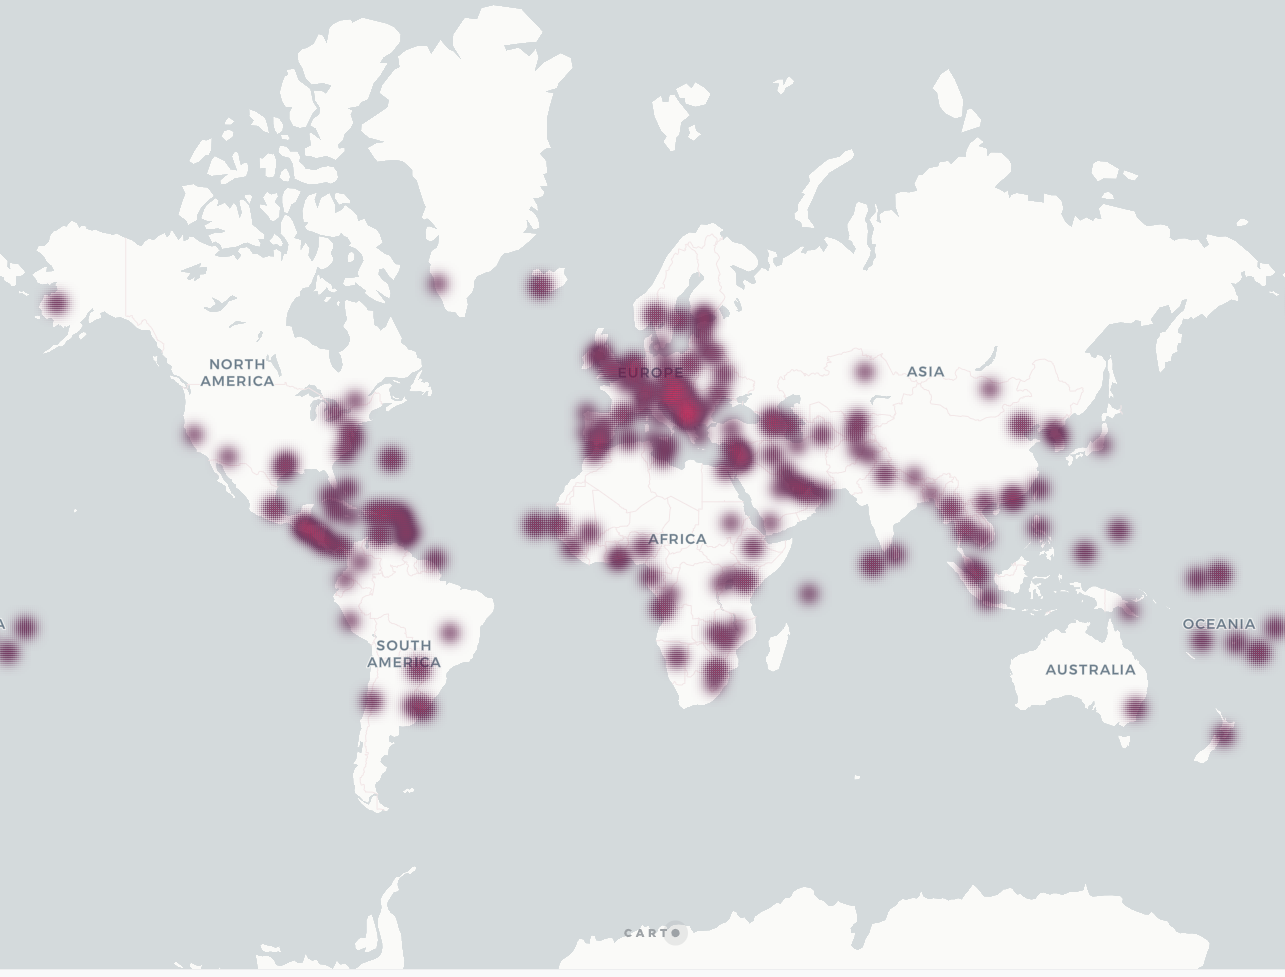
\includegraphics[width=0.95\textwidth]{images/Mapa_calor_FC.png}
    \caption[1]{Fuente: \url{https://clausa.app.carto.com/map/f16b7877-40d4-4182-8c3e-043b5bdb2aa2}}
\end{figure}

\textbf{Tipo de mapa:} Mapa de calor (heatmap) \\
\textbf{Ubicación en el espectro de mapas:} Cuantitativo – Distribución espacial de densidad por unidad política (país). \\

\textbf{Esquemática:} \\
\begin{itemize}
    \item \textit{Descripción:} Visualización de la concentración de incidentes cibernéticos registrados entre 2014 y 2024 por país.
    \item \textit{Secuencia:} Se partió desde el dataset completo, se agrupó por país y se contó la cantidad de incidentes. Se añadieron coordenadas geográficas y se cargó el resultado a CARTO como mapa de calor.
\end{itemize}

\textbf{Colores utilizados:} \\
Se utilizó una paleta monocromática que va desde blanco a rojo oscuro. Esta elección refuerza la percepción de urgencia y riesgo en zonas con alta concentración de incidentes.

\textbf{Tipografía empleada:} \\
CARTO emplea una tipografía sans-serif clara, de alto contraste, que mantiene coherencia con el diseño minimalista de la plataforma. Esto permite que el foco esté en los datos visualizados y no en elementos distractores.



\vspace{1em}
\subsection*{Mapa 3: [Título del compañero 2 (Kepler.gl / Tableau / etc)]}
\textit{[Espacio para que tu compañer@ agregue imagen, enlace y detalles según pauta]}


% ===================== INTEGRANTE 1 =====================
\section*{Análisis por Integrante}

\subsection*{Integrante 1: Javier Gomez}


\subsubsection*{Gráfico 1: Mapa de puntos categorizados}
\begin{figure}[H]
    \centering
    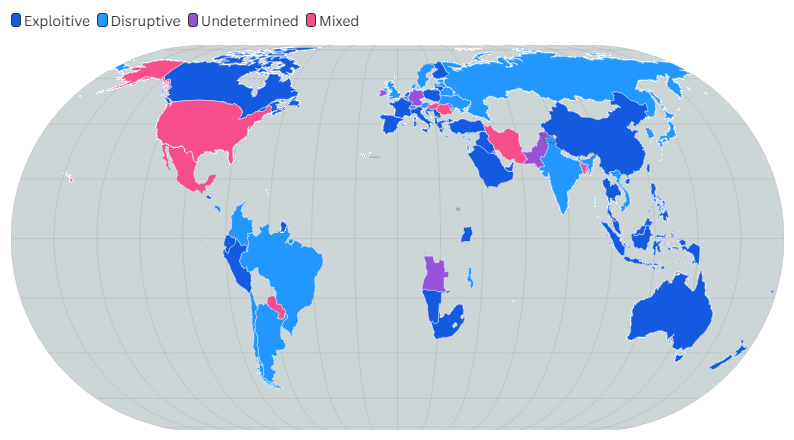
\includegraphics[width=0.9\textwidth]{images/punto_cate.png}
    \caption{Fuente: Elaboración propia con datos}
\end{figure}

\paragraph{Descripción cualitativa del dataset:}

El conjunto de datos contiene información sobre ataques cibernéticos dirigidos a diferentes países. Cada registro describe:
\begin{itemize}
    \item El tipo de actor que realiza el ataque (por ejemplo, \textit{Nation-State}, \textit{Criminal}).
    \item El motivo del ataque (\textit{Sabotage}, \textit{Financial}, etc.).
    \item El tipo de evento (\textit{Exploitive}, \textit{Disruptive}, etc.).
    \item El país objetivo del ataque.
\end{itemize}
Esta información permite clasificar a los países según el tipo de ataque más común que han recibido, representado gráficamente en el mapa mediante distintos colores.

\paragraph{Objetivo de la visualización:}

\begin{itemize}
    \item \textbf{¿Qué pregunta busca responder?} \\
    ¿Qué tipo de ataques cibernéticos predominan en cada país y cómo se distribuyen globalmente?

    \item \textbf{¿A qué público está dirigida?} \\
    A responsables de ciberseguridad, analistas de riesgos, académicos y tomadores de decisiones en políticas públicas.

    \item \textbf{¿Qué acción o decisión podría apoyar?} \\
    Esta visualización puede ayudar a:
    \begin{itemize}
        \item Identificar patrones geográficos de ciberataques.
        \item Establecer prioridades de protección en función del tipo de amenaza.
        \item Fomentar cooperación internacional en ciberseguridad.
    \end{itemize}
\end{itemize}

\paragraph{Conclusiones:}
\begin{itemize}
    \item La mayoría de los países presentan ataques del tipo \textbf{Exploitive}, lo que indica una tendencia a aprovechar vulnerabilidades sin necesariamente causar interrupciones.
    \item Algunos países, como Estados Unidos, muestran una predominancia de ataques \textbf{Disruptive}, que buscan causar interrupciones o daños visibles.
    \item Aparecen categorías \textbf{Mixed} o \textbf{Undetermined} en países donde hay múltiples tipos de ataques o falta de información clara.
    \item Existe una correlación geopolítica: regiones con conflictos o tensiones políticas muestran ataques más agresivos o frecuentes, como en el caso de Ucrania e Irán.
\end{itemize}
\subsubsection*{Anexo: Ataques saboteadores por actores estatales}
\begin{figure}[H]
    \centering
    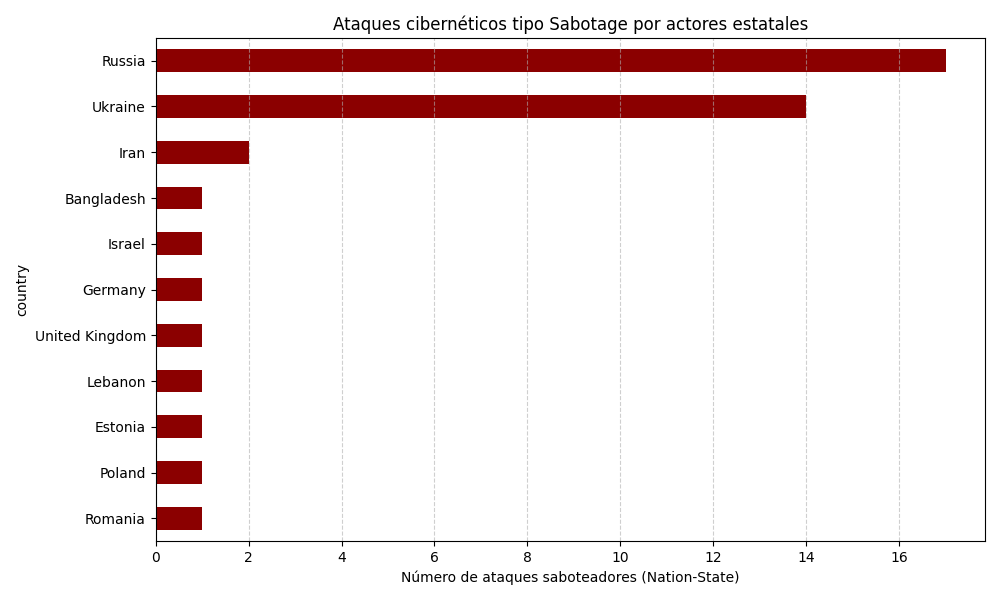
\includegraphics[width=0.8\textwidth]{images/sabotage_state.png}
    \caption{Ataques cibernéticos con motivo de sabotaje realizados por actores estatales. Fuente: Elaboración propia con datos del dataset.}
\end{figure}



\subsubsection*{Gráfico 2: [Nombre del gráfico]}
\begin{figure}[H]
    \
\end{figure}

\textbf{Conclusión:}
\begin{itemize}
    \item ...
\end{itemize}

% ===================== INTEGRANTE 2 =====================
\newpage
\subsection*{Integrante 2: Felipe Campaña}

\subsubsection*{Mapa 2: [Mapa de Calor en CARTO]}
\begin{figure}[H]
    \centering
    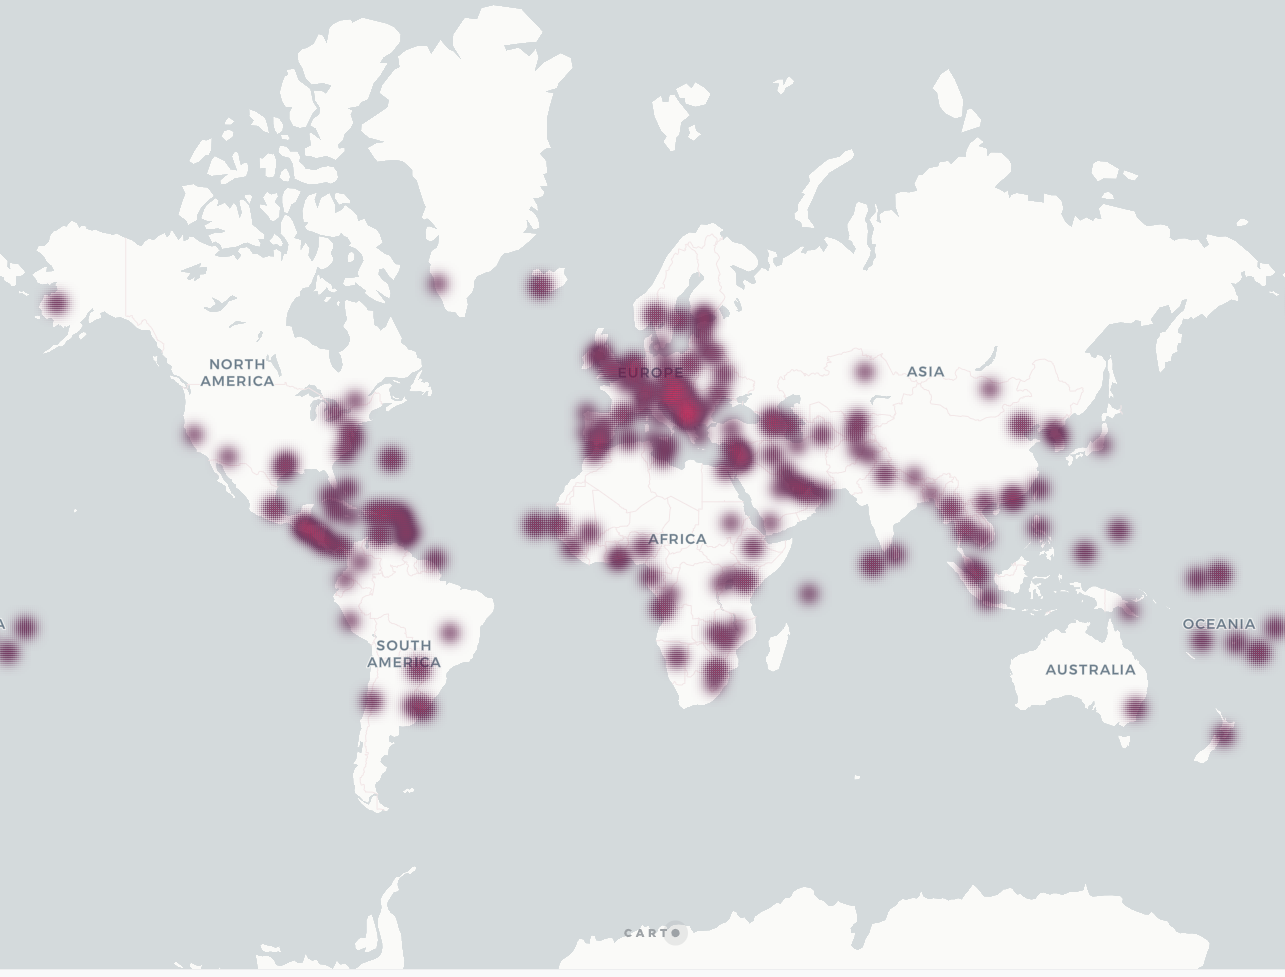
\includegraphics[width=0.85\textwidth]{images/Mapa_calor_FC.png}
    \caption[1]{Fuente: \url{https://clausa.app.carto.com/map/f16b7877-40d4-4182-8c3e-043b5bdb2aa2}}
\end{figure}

\textbf{Descripción cualitativa del dataset:} \\
El dataset utilizado proviene de la base de datos \textit{Cyber Events Database (2014–2024)} de la Universidad de Maryland. Esta base documenta más de 14.000 eventos de ciberseguridad relevantes a nivel mundial, incluyendo país afectado, tipo de ataque, actor responsable, sector y fecha. Se procesó agrupando los datos por país víctima para contar la cantidad de incidentes por ubicación geográfica.

\vspace{0.5em}
\textbf{Objetivo de la visualización:} \\
\begin{itemize}
    \item \textit{¿Qué pregunta busca responder?} \\
    ¿En qué países se han concentrado más ciberataques registrados entre 2014 y 2024?
    
    \item \textit{¿A qué público está dirigida?} \\
    Principalmente a periodistas de datos, investigadores en ciberseguridad y tomadores de decisiones en políticas públicas tecnológicas.

    \item \textit{¿Qué acción o decisión podría apoyar?} \\
    Esta visualización permite identificar regiones con alta exposición a amenazas cibernéticas, ayudando a priorizar recursos en ciberdefensa, programas de concientización o cooperación internacional.
\end{itemize}

\vspace{0.5em}
\textbf{Tipo de visualización:} \\
Mapa de calor (\textit{Heatmap}) realizado con la plataforma CARTO. Representa la densidad de incidentes cibernéticos según país. Mientras más rojo concentrado, mayor es la cantidad de eventos registrados en esa región.

\vspace{0.5em}
\textbf{Justificación de diseño:} \\
\begin{itemize}
    \item \textbf{Colores:} Se utilizó una escala monocromática rojo oscuro $\rightarrow$ blanco. El rojo transmite alerta, urgencia y riesgo, reforzando el mensaje de amenaza.
    \item \textbf{Tipografía y estilo:} CARTO aplica tipografía clara sin ruido visual. Se privilegia la lectura del mapa más que el texto.
    \item \textbf{Geocodificación:} Se asignaron coordenadas geográficas centrales a cada país para representar los datos en el mapa.
\end{itemize}

\vspace{0.5em}
\textbf{Conclusiones del gráfico:} \\
\begin{itemize}
    \item América del Norte, Europa Occidental y partes de Asia (China, Corea del Sur, India) son focos principales de ciberataques.
    \item Hay una notable concentración en países desarrollados, lo que puede asociarse tanto a mayor exposición tecnológica como a mejor capacidad de reporte.
    \item Regiones como África y Oceanía muestran baja densidad, aunque esto puede deberse a subregistro o menor cobertura mediática.
    \item El mapa permite hacer inferencias sobre la correlación entre infraestructura digital y volumen de ciberincidentes.
\end{itemize}

% ===================== INTEGRANTE 3 =====================
\newpage
\subsection*{Integrante 3: Nombre del estudiante}

% Repite la misma estructura

% ---------------------------------------------------------------------------------
\section{Evidencia de encuesta aplicada}
Aquí puedes insertar una imagen de la base de datos, resumen de resultados o archivo fuente.

\begin{figure}[H]
    \centering
    \caption{Captura de pantalla del archivo Excel con las respuestas de la encuesta}
\end{figure}


\textbf{Repositorio:}  
\label{anexo:repositorio}

Acceso al repositorio en el siguiente link:  
\url{https://github.com/usuario/repositorio.git}

\end{document}
